\documentclass{article}

\usepackage[hidelinks]{hyperref}
\usepackage{enumitem}
\usepackage{todonotes}
\usepackage{listings}
\usepackage{color}
\usepackage[plain]{fancyref}
\usepackage{subfigure}
\usepackage{wrapfig}
\usepackage{float}
\usepackage{graphicx}
%\usepackage{marginnote}
%REMOVE BELOW COMMAND TO GET NORMAL VIEW
%\usepackage[top=1.5cm, bottom=1.5cm, outer=5cm, inner=2cm, heightrounded, marginparwidth=2.5cm, marginparsep=2cm]{geometry}

\definecolor{light-gray}{gray}{0.95}
\lstset{mathescape,
		basicstyle=\ttfamily,
		backgroundcolor=\color{light-gray}
		}
\lstset{numbers=right, 
                numberstyle=\tiny,
                escapechar=\&,
                breaklines=true,
                backgroundcolor=\color{light-gray},
                %xleftmargin=\parindent,
                %xleftmargin=1cm,
                %xrightmargin=\parindent,
                numbersep=5pt}

%\newcommand*{\UTlogo}{\fbox{$\mathcal{UT}$}}
\newcommand*{\UTlogo}{
\includegraphics{Figures/utlogo.png}}

%---------------------------------------------------------------------------
%	TITLE PAGE
%	Page taken from: http://www.latextemplates.com/template/vertical-line-title-page
%---------------------------------------------------------------------------
\newcommand*{\titleGM}{\begingroup
\hbox{
\hspace*{0.2\textwidth}
\rule{1pt}{\textheight}
\hspace*{0.05\textwidth}
\parbox[b]{0.75\textwidth}{

%{\noindent\LARGE \textit{Note: Margin notes version!} \\ \textit{Note: Spell check should be done!} } \\[2\baselineskip]
{\noindent\Huge\bfseries Stairwalker \\[0.5\baselineskip] User Manual}\\[2\baselineskip]
%{\large \textit{We could write something here}}\\[4\baselineskip]
{\Large \textsc{Dennis Muller} \\[0.25\baselineskip]
 \Large \textsc{Jochem Elsinga} \\[0.25\baselineskip]
 \Large \textsc{Maurice van Keulen}}

\vspace{0.1\textheight}
{\noindent\fbox{
\includegraphics{COMMIT_logo_RGB.pdf}}}

\vspace{0.3\textheight}
{\today}\\
{\noindent \UTlogo}\\[\baselineskip]
}}
\endgroup}

%---------------------------------------------------------------------------
%	DOCUMENT
%---------------------------------------------------------------------------
\begin{document}

\pagestyle{empty}

\titleGM

\tableofcontents
\pagebreak
\pagestyle{plain}
%---------------------------------------------------------------------------
%	Sections
%---------------------------------------------------------------------------

\section{Introduction}
Geographical data are typically visualized using various information layers
that are displayed over a map. Interactive exploration by zooming and
panning actions needs real-time re-calculation. A common operation in
calculating with multidimensional data is the computation of aggregates.
For layers containing aggregated information derived from voluminous data
sets (see for example Figure~\ref{fig:NL-screenshot}), such real-time
exploration is impossible using standard database technology. Calculations
require too much time.

The University of Twente has developed \emph{``Stairwalker''}: database
technology that accurately aggregates data so that they can geographically
be explored in real-time. The technology is a plug-in to common open
source technology.

Its core is the \emph{pre-aggregate index}: a database index that cleverly
pre-calculates aggregation values such that it can obtain exact aggregation
results from voluminous data with high performance.  A fast calculation
allows to fully recalculate the result for even the slightest movement of
the map, such as a panning or zooming action, without loss of accuracy.
Thanks to this indexing mechanism, we can provide a scalable real-time
calculation: an order of magnitude larger dataset requires only one
additional aggregation level.

In geo data visualization, the ability to quickly develop new information
layers is important. Although many solutions exist, there is a niche: the
combination of visualizing aggregation information, interactive data
exploration in real-time, Big Data, calculating exact numbers instead of
approximations, and doing so with common open source technology. Our
technology for the first time integrates all these features.

\begin{figure}[t]
\centering
\includegraphics[height=4in]{Figures/NL-screenshot.pdf}
\caption{Twitter hotspot detection in The Netherlands, using a coarse grid.
The numbers inside the grid cells on the map require an aggregation
operation in the database.}
\label{fig:NL-screenshot}
\end{figure}


Our research partners are the companies Arcadis and Nspyre. They both have
struggled with this combination of requirements in many of their projects.
Our database index technology is not specific to geographical data. It can
be used with all types of multidimensional data. Visualization in business
intelligence or eScience can also benefit from it.

\begin{figure}[t]
\centering
\includegraphics[width=4in]{Figures/DCMR-screenshot.pdf}
\caption{Tweets about excessive smells in the vicinity of the Rotterdam
harbor}
\label{fig:DCMR-screenshot}
\end{figure}

\paragraph{Nice to know}
The company Arcadis developed an application for the DCMR Milieudienst
Rijnmond based on the Stairwalk technology to investigate whether people
send tweets about unpleasant odors as a possible signal of danger (see
Figure~\ref{fig:DCMR-screenshot}). This turns out not to be the case,
probably because people think that nobody reads the tweets anyway. But if
people have the idea that their complaining tweets are read, then tweets
might be much more convenient than the reporting of unpleasant odors by
telephone.

\paragraph{This manual}

This manual explains how to use Stairwalker.  We first explain in
Section~\ref{sec:setup} how to install the required components in order to
have a basic running system.  We then explain in
Section~\ref{sec:deployment} how to add databases and different kinds of
datatypes to Geoserver, an open source server for sharing geospatial
data.\footnote{\url{http://geoserver.org}} It is explained how to show and
customize layers and views, but also how to adjust the system, for example,
how to add dimensions or use different dimension types such as median.
Finally, Section~\ref{sec:development} explains how to extend the system.

\paragraph{Acknowledgements}

This publication was supported by the Dutch national program COMMIT/.

\pagebreak
\section{Set Up}
\label{sec:setup}
In this section a detailed description will be given about setting up all the required peripheral programs to use stairwalker.

\subsection{Database Setup}
At the moment the Stairwalker program only works with the PostgreSQL\footnote{PostgreSQL: \url{http://www.postgresql.org}} and MonetDB\footnote{MonteDB: \url{http://www.monetdb.org}} database management systems. This manual will only concern itself with PostgreSQL (shortened to Postgres). Any further reference to a database implies a Postgres database.

In this section a walk through explaining the steps needed to setup PostgreSQL along with PostGIS\footnote{PostGIS: \url{http://www.postgis.net}} and a custom made database extension for Stairwalker on an Ubuntu Linux kernel.

\subsubsection{PostgreSQL Database Manager Setup}
Installing Postgres on Linux should be straight forward. In the terminal search for Postgresql and then choose which version of Postgresql should be installed. Below the commands used to search and install version 9.1 of Postgres are shown.
\begin{enumerate}
	\item \lstinline|aptitude search postgresql|
	\item \lstinline|apt-get install postgresql-9.1|
\end{enumerate}
For further information or if there are difficulties with the installation more details can be found on the installation page of the \href{http://www.postgresql.org/download/}{PostgreSQL website}.  

\subsubsection{PostgreSQL Configuration}
Once Postgres is installed on Linux two alterations will need to be made to the configuration files so that the database can be accessed from outside and by other users.

First off in the \lstinline|Postgresql.conf| file the listen\_addresses need to be changed from localhost to all. This can be done as follows (assuming version 9.1 of Postgres).

\begin{enumerate}
	\item \lstinline|cd /etc/postgresql/9.1/main|
	\item \lstinline|vi postgresql.conf|
	\item \textit{change} listen\_addresses = `localhost' $\rightarrow$ listen\_addresses = `*'
	\item \textit{save and close}
\end{enumerate}

\noindent Secondly in the file \lstinline|pg_hba.conf| a line needs to be added to allow other users in Linux to access postgres. This can be done as follows:

\begin{enumerate}[resume]
	\item \lstinline|vi pg_hba.conf|
	\item \textit{Add} host all	all 0.0.0.0/0 password
	\item \textit{save and close}
	\item \lstinline|/etc/init.d/postgresql restart|
\end{enumerate}

\noindent It should now be possible to create a database user and database in Postgres. More information about how this is done can be found on the \href{http://www.postgresql.org/docs/manuals/}{Postgres manuals webpage}.

\subsubsection{PostGIS Configuration in PostgreSQL}
The next step is to extend Postgres with PostGIS database expansion. This again should be straight forward, first search for PostGIS and then choice the version that goes with Postgres to install. Note in order to do the install root privileges are required. Below the commands to search and install PostGIS for Postgres-9.1 are shown.

\begin{enumerate}
	\item \lstinline|aptitude search postgis|
	\item \lstinline|apt-get install postgresql-9.1-postgis|
\end{enumerate} 

\noindent More information about installing PostGIS  can be found on the \href{http://www.postgis.net/install}{PostGIS website}.
\newline
\newline
%I am not so sure why this is done or if it is even neccesary.
Once PostGIS is installed some extra configuration is required. This needs to be done as postgres user. The commands are as follows.

\todo[inline, size=\small]{Why do we do this again? What does it do?}
\begin{enumerate}	
	\item \lstinline|createlang plpgsql geonames|
	\item \lstinline|psql -f `find/usr/share/postgresql/ -name postgis.sql -print' -d geonames|
	\item \lstinline|psql -f `find/usr/share/postgresql/ -name spatial_ref_sys.sql -print' -d geonames|
	\item \lstinline|psql -f `find/usr/share/postgresql/ -name postgis_comments.sql -print' -d geonames|
\end{enumerate}

\subsubsection{Serverside Stairwalker Extension in PostgreSQL}
\label{sec:serversideextension}
Finally there is C extension which allows processing of the SQL queries for the pre-aggregated database to happen on the server side instead of in the GeoServer application. This extension has to be installed on the Postgres database. The extension can be found in the directory \lstinline|neogeo/pre-aggregate/src/db-extensions/postgres/pa_grid|.

The extension can be installed on Linux using the following commands.

\begin{enumerate}
	\item \textit{go to the pa\_grid\ directory in the terminal}
	\item \lstinline|make| \\ \textit{this creates the dynamic library}
	\item \lstinline|make install| \\ \textit{this installs the library in the postgres installation}
	\item \lstinline|make sql| \\ \textit{declare the module in the database wanted}
\end{enumerate}

\noindent\textbf{Note} the extension has to be installed specifically for the database which will be used for pre-aggregation. In the makefile (also in the \lstinline|pa_grid| folder) there is a \lstinline|DATABASE| macro which should be set to the desired database.

\todo[inline, size=\small]{Installing the extension also requires root access. Why was this again?}


\subsection{Pre-Aggregate Database Table}
\subsubsection{Description of Process}
Stairwalker makes use of the Pre-Aggregate functions. These functions create a granularity in the dataset and calculate blocks at the lowest granularity for certain dimensions. Then subsequent blocks of higher granularity are built up from lower blocks. This creates a new dataset which as summarized the original dataset in terms of blocks which represent some significant data for every level of granularity and dimension.

%Is dit duidelijk? Klopt dit eigenlijk??
%Nog iets met index of zo...
Concretely take the dataset of tweets sent within the netherlands. A pre-aggregation of this data could be in the following form. As significant data we consider the number of tweets in the x- and y-coordinate dimensions. We then set a highest granularity (zoom). The pre-aggregate algorithm then creates blocks bounded by the x- and y-coordinates at the highest granularity and for all those blocks calculates the number of tweets within those coordinates. Then each subsequent layer is built up from the previous layer. The final result is a new dataset which contains all blocks with the number of tweets in a coordinate block at each level of granularity.

\subsubsection{PreAggregate Tool}
To do the Pre-Aggregation step a tool has been develped which is explained here.

\noindent The tool can be found in the directory \lstinline$neogeo/pre-aggregate-tools/$. To generate the binary tools from source the Appassembler plugin of Maven is used. Run the following command to generate the tool.
\begin{lstlisting}
mvn package appassembler:assemble
\end{lstlisting}
After successful completion of this command a new directory \lstinline$appassembler$ will have been created in the \lstinline$target$ directory containing a \lstinline$repo$ and a \lstinline$bin$ directory. The \lstinline$bin$ directory contains the actual binaries of the tool (in both Linux/Unix and Windows version) and the \lstinline$repo$ directory contains the tool dependencies. The tool should now be ready for use.

The tool is used to create a PreAggregate index for a table with $\textit{n}$ dimensions and a measure/aggregate column. It uses with the following commands:
\begin{lstlisting}[basicstyle=\small]
usage: create-pa-index
 -axistosplit <axis index>    index of axis to split
 -chunksize <size>            maximum chunk size after split
 -config <file>               PreAggregate XML config file
 -d,--database <dbname>       name of database
 -dbtype <postgresql|monetdb> type of database
 -h,--host <host>             database host name or ip address
 -help                        prints this help message
 -p,--port <port>             port number of the database
 -password <password>         database password
 -s,--schema <schema>         schema name in the database
 -u,--user <user>             database username
 -v,--verbose                 Enable verbose output logging
\end{lstlisting}
The tool is dependent on the \lstinline$PreAggregate.XML$ config file which is used to define the PreAggregate index by specifying the column to aggregate, the type of aggregate that should done and the dimensions to include. In the \lstinline$neogeo/pre-aggregate-tools/$ directory a sample configuration file is included.

\todo[inline, size=\small]{How does this tool work nominal axis? More preprocessing may be required when first parsing words? Example london\_words or gender\_words}

see~\Fref{sec:PreAggregateDev} for more detail about preaggregation not using the special help tool.

Apart from creating a new PreAggregate table \lstinline$<original-table-name>_pa$ pre-aggregation also creates/updates two other tables, these are \lstinline$pre_aggregate$ and \lstinline$pre_aggregate_axis$. These two tables are support tables for the aggregation. They contain information about which tables have been aggregated and which axis have been used in pre-aggregation.
\subsubsection{Current Status Support of Datatypes}
\begin{enumerate}
	\item Aggregate Axis
	\item Metric Axis
	\item Nominal Axis
\end{enumerate}

\subsubsection{Current Status Support of Aggregation Types}
At the moment you can aggregate your data in a total of 4 options and all 4 options have a different outcome.

The options that you can use at the moment are the following:
\begin{enumerate}
\item ALL: 	???
\item Count: returns the total amount of data in an aggregate box. Returns a number with the total amount of that tile.
\item Sum: returns the total value of all data added up to eachother. For instance when you do a sum on the tweet length you'll get the total amount of characters tweeted in a tile.
\item Min: returns the lowest value of all data that is aggregated. With the example of tweet length, it will returns the value of the lowest length tweet in that tile.
\item Max: returns the highest value of all data that is aggregated. With the example of tweet length, it will returns the value of the highest length tweet in that tile.
\end{enumerate}

It is important to chose the right type in order to get a good representation of your data. If you want to show the total amount in a tile, you should chose count as this will returns the total number of tweets in a tile. Whereas if you want only the highest value of your data (for example the highest building in an area) then it is important to use max. It is also possible to add other datatypes than the onces mentioned here. To do so check the section about development, here you will find more information about how to add a different aggregation type.


\subsection{Tomcat Server Setup}
\textbf{Information about how to setup a web server (tomcat).}
\label{sec:tomcat}

\subsection{Geoserver Deployment on Tomcat}
\textbf{Information about how to setup and deploy the geoserver .war file in tomcat.}

\pagebreak
\section{Deployment}
\label{sec:deployment}
This section will give a detailed description of how to import an aggregated database table into GeoServer to get a visual representation of the dataset. First instructions will be given on how to link the database table to GeoServer. Next creating styles and layers for data representation will be discussed. The final sub section will discuss how to view the data using GeoServer.  For this section it is assumed that all the initial preparation discussed in \Fref{sec:setup} has been completed.\\newline

GeoServer should already be deployed on a web server (see \Fref{sec:geotomcat}), and can then be accessed with \lstinline|http://<Tomcat-IPaddress>:8080/geoserver/web/|. It is required to login in to the GeoServer administration interface. When using the default setup of GeoServer the login credentials are: \\
\indent \textbf{username:} admin \\
\indent \textbf{password:} geoserver

\subsection{Add Source}
%Once the webapplication has logged in, then start by adding the source of the database. 
%\begin{enumerate}
%	\item On the left side there should be a menu with all kinds of options, but in order to add a source, go to Configuration $\rightarrow$ Sources. 
%	\item At the top there should be an add source button. 
%	\item Now under vectortypes there should be a list of types. Select what kind of source you want to add. In order to get the Stairwalker program running there should be a NeoGeo Aggregate - NeoGeo aggregation index query. If this is not the case something went wrong with deploying the geoserver and the last steps in this manual should be done again. 
%	\item If it is here, click on it and a new menu will open. A new screen should open where all information for your source has to be filled in. There is also an option on what aggregation type the program should use, this should have been defined before so use what has been used before (count/sum/minimum/maximum). 
%	\item Once everything is filled in all, the source should have been added to the Geoserver. This can be checked by going to sources again and then it should display the source that has just been added.
%\end{enumerate}

Once logged in to the web administration interface it is possible to add a new data store to GeoServer. Instructions of how to add a new \lstinline|NeoGeo Aggregate| vector data source which contains the aggregate index created in \Fref{sec:preaggtool} to the stores in GeoServer.

\begin{enumerate}
	\item Navigate to \lstinline|Stores| by clicking on \lstinline|Stores| link under the \lstinline|Data| section in the navigator on the left hand side of the web administration interface homepage.
	\item On the \lstinline|Stores| page select the option \lstinline|Add new Store| located at the top of the page. This leads to a page titled \lstinline|New Store chooser|.
	\item In the list of \lstinline|Vector Data Sources| the option \lstinline|NeoGeo Aggregate| should be present, choose this format for the data source.  
\end{enumerate}

\noindent If the option \lstinline|NeoGeo Aggregate| is not available it means the GeoServer extension from \Fref{sec:InstallExtension} was not done correctly.

\begin{enumerate}[resume]
	\item Clicking \lstinline|NeoGeo Aggregate| will open a new page titled \lstinline|New Vector Data Source| in which several fields have to be filled out, explanation of mandatory fields can be found in the list below on page \pageref{list:manditory}.
	\item For an express setup the fields which have already been filled can remain the same.
	\item Once all the required fields are filled in click the \lstinline|Save| button.
	\item A new \lstinline|NeoGeo Aggregate| source is now created and can be view and edited in \lstinline|Sources|.
	\item After saving GeoServer opens the page \lstinline|New Layer| on which new layers can be created using the \lstinline|Data Source|. How this is done is discussed in \Fref{sec:addinglayers}.
\end{enumerate}

\noindent Here a list of all mandatory fields on the \lstinline|New Vector Data Source| page with explanation.

\begin{itemize}\label{list:manditory}
	\item \textbf{Data Source Name} - An arbitrary name which will be assigned to the store.
	\item \textbf{Database type} - The type of underlying database, either PostgreSQL or MonetDB.
	\item \textbf{Hostname} - Hostname of the database server where the aggregation index is maintained.
	\item \textbf{Port} - Port number of the database.
	\item \textbf{Schema} - Name of the schema where the aggregation index is maintained.
	\item \textbf{database} - Name of the database where the aggregation index is maintained.
	\item \textbf{Username} - Username of the used database.
	\item \textbf{Password} - Password of the used database.
	\item \textbf{xSize, ySize, timeSize} - Specifies the dimensions of the grid which is created for every view of the map to calculate the aggregates per cell. The higher the number of cells the more detailed the information. \\
	\todo[inline, size=\small]{Are the xSize, ySize, timeSize dimensions not already set in the source? What happens when timeSize $< 1$?}
	\item \textbf{count, sum, minimum, maximum} - Select the boxes of the aggregates which will be used in the visualization. Note that these basic aggregates more aggregates such as mean can can be derived.
	\item \textbf{Enable server-side Stairwalker} - Selecting will cause the data source to rely on the use of the database plugins to use the Pre-Aggregate index. For performance reasons it is high recommended to use this option. See \Fref{sec:serversideextension} for more details.
	\todo[inline, size=\small]{The Enable server-side Stairwalker ooption is no longer avaible? Remove?}
	\item \textbf{Enable query logging} - Selecting will turn on the logging of all Pre-Aggregate queries into a separate table called \lstinline|pre_aggregate_logging|.
\end{itemize}
\pagebreak

\subsection{Setup Style}
%The next step is to make a style in which you want your data to be shown. A style has to be made in SLD/XML, there are a lot of options which can be used to make a style. First navigate to the style tab, Configuration $\rightarrow$ Style here you can add a new style with the button on top. Here you need to add your code (or file) for your style.
%\newline
%\newline http://docs.geoserver.org/2.5.x/en/user/styling/sld-cookbook/index.html contains a lot of information regarding styles, it is a lot of trial and error to get a nice working style. The next few steps however should give a short setup on how to start making your own style.
%\begin{enumerate}
%	\item Decide what data should be shown, in our example we’re using the count of the aggregated data.
%	\item Decide what kind of representation should be used, you can either use Polygonsymbolizer, pointsymbolizer or linesymbolizer. All of these have their own advantages and disadvantages, incase it isn't clear what to use, start off with a Polygonsymbolizer.
%	\item Add all filters, for instance if the data should how a lighter color if the amount is lower. Or make a tile red once the data exceed a certain maximum (for instance if there were too many orders in a timerange).
%	\item Add colors to the layers representing it better and giving it a nice layout.
%	\item Make sure the positioning of the label and all filters are working.
%	\item Finish the layer by adding the last details (Halo behind the text for example).
%\end{enumerate}
%
%This is just a basic manual on how to add a style, for more information or more explanation on how to make a style, check out the development chapter in this manual. In that section there are far more details on how to make a style.
%

In GeoServer, styles are used to render, or make available, geospatial data.
Styles are used to visually represent the aggregation index which is
represented in a layer. In GeoServer layers are written in Styled Layer
Descriptor (SLD) which is a subset of XML. GeoServer comes setup with
several different styles, however, to get the most out of the dataset it is
best to develop a style specific to the layer which represents that data.

In this section only instructions on how to add new styles to GeoServer are
given. For information on how to edit styles, see \Fref{sec:visualization}
or the GeoServer user
manual\footnote{\url{http://docs.geoserver.org/stable/en/user/styling/index.html\#styling}}
which gives an in depth guide on developing styles.

\begin{enumerate}
	\item Navigate to \lstinline|Styles| by clicking on the \lstinline|Styles| link under the \lstinline|Data| section in the navigator on the left hand side of the web administration interface homepage.
	\item On the \lstinline|Styles| page select the option \lstinline|Add a new style| located at the top of the page.
	\item A new page titled \lstinline|New Style| should open. There are now two possibilities, either a new style can be developed completely in the browser or a SLD file can be imported.
	\item To import an already created SLD file scroll to the bottom of the page and press the \lstinline|Choose File| button.
	\item Select the style which should be imported and then press \lstinline|Upload...| in the browser.
	\item This fills in the \lstinline|Name| field with the name of the file and the SLD editor with the content of the file.
	\item It is possible to check the syntax of the SLD code by pressing the \lstinline|Validate| button at the bottom of the page. At the top the page GeoServer will give feedback on the SLD code, either error messages or a no validation errors message.
	\item Finally the style can be saved by pressing the \lstinline|Submit| button at the bottom of the page.
\end{enumerate}
%\todo[inline, size=\small]{We should maybe mention something about the workspace? What does \lstinline|nurc| represent? It is even important to choose a workspace?}


\subsection{Adding Layer}
Now we have a source and have a style to use, it is time to setup a layer to display this style. 
\begin{enumerate}
	\item Go to Configuration -> Layers and press the button on top, you should get a dropdown menu in which you need to select your database. Once you've done this it should show the data which can be displayed. 
	\item Select the data you want and press Publish. You'll need to fill in all these fields in order to get the layer to work. Important are the projections. In our layers we use Projection of Source, EPSG:4326, and Given Projection, EPSG:3587. We set handling of the projection to use the given projection. Then for Boundary Rectangles let them be calculated based on sourceprojection. And then all fields should be filled in, do not press save yet however. 
	\item On top select publish. Here you can select the style you want to be used in order to display your data, select your own style here. \item Once this is done you can press save and your layer should be added.
\end{enumerate}


\subsection{On Client (html page) Link Geoserver + Layer}
%Now in order to see the layer go to view, here it should display the layer that has been made (with the added name) with a drop-down menu. Select PNG/JPEG or something similar to show a basecase of the data. A new window should open and here it should show your data in a weird graph. If this is not the case, its likely a mistake in the style. It is also possible to adjust your view in the images by adding a VIEWPARAM to the url. To do so just add: \&VIEWPARAMS=$<$Type$>$:$<$Value$>$ to the url and the image should change.

In GeoServer it is possible to get a preview of layer such as the one created in \Fref{sec:addinglayers}. Previewing a layer can be done as follows:

\begin{enumerate}
	\item Navigate to \lstinline|Layer Preview| by clicking \lstinline|Layer Preview| link under the \lstinline|Data| section in the navigator on the left hand side of the web administration interface homepage.
	\item The \lstinline|Layer Preview| page will have a list of all configured layers with can be previewed in various formats.
	\item Locate the layer which should be shown and from the \lstinline|All Formats| column choice any \lstinline|WMS| format.
	\item After selecting a format to view the layer a new page will open with a visual representation of the top most layer of dataset.
\end{enumerate}

Note that other preview formats should also be possible. For example it is possible to use the OpenLayers preview format which allows one to navigate the geospatial data. In section \Fref{sec:clientsidedev} OpenLayers will also be used to visualize the dataset on a web page. One drawback is that for every movement in the preview a new query has to be calculated. When server side stairwalker (\Fref{sec:serversideextension}) is not setup calculating can be time consuming. Therefore during development of the pre-aggregation index and testing it is advices to use a static preview and only once everything works as desired to use a dynamic preview.

If the layer contains a nominal axis it is possible to alter the value of the nominal with which the data is filtered. This is done by adding a parameter in the request made to the GeoServer extension. By extending the \lstinline|HTML| request sent to GeoServer with \lstinline|&VIEWPARAMS=<TYPE>:<VALUE>;| the nominal axis filter is used. Currently the extension only supports the nominal type \lstinline|keyword|. If the pre-aggregate index was created using a nominal axis (splitting on \lstinline|VALUE|s) then using \lstinline|&VIEWPARAMS| will split the visualization on a give \lstinline|VALUE|. \lstinline|&VIEWPARAMS| can accept more \lstinline|<TYPE>:<VALUE>;| tuples, however parsing type will need to be extended on in the code. For more information see \Fref{sec:filtering}.

It may be that a preview fails to load, this can be due to two reasons. The first is an error in the style, in this case the style needs to be tested which can be done by validating the style in GeoServer. For more information about styles see \Fref{sec:visualization}. The second reason is an error is creating an SQL query for the pre-aggregated index. If no mistakes where made during setup and in creating a pre-aggregate index there will be a need to dive into the code where detailed logging is done.
\todo[inline, size=\small]{This would be a good point to reference the logging done in the code however i cannot find where this log file is located, debugging is also possible using the console in an IDE.}



\pagebreak
\section{Development}
\label{sec:development}
\subsection{Code Development}
\label{sec:PreAggregateDev}
In this section some pointers will be given to important sections of code in terms of processing pre-aggregate indexes which are used by the GeoServer extension.

\subsubsection{Filtering Words for Nominal Axis}
\todo[inline, size=\small]{This subsection should deal with filtering the GET request sent to GeoServer making the \&VIEWPARAMS work as desired. Also maybe other things with time or other axis??}


\subsubsection{Creating Pre-Aggregate Index from Source}
\todo[inline, size=\small]{This subsection should deal with creating a pre aggregate index using source code, this means defining ones own axis, pre-processing in terms of nominal axis and pointing to the right tables/column etc.}
\pagebreak

\subsection{Geoserver Visualization}
\label{sec:visualization}
This section is going to discuss most of the possibilities that Geoserver has to offer when it comes to the visualization of the data. The GeoServer manual has some information on this subject, which can be found here;

\url{http://docs.geoserver.org/2.5.x/en/user/styling/sld-reference/index.html}

The following sections will give some more information on what the differences are between the different options and some ways to implement the different options. This section will use some of the examples used in our demo to give some more insight what can be done and hopefully making it easier to realise what is wanted. Most information can be found on the website, below will be a discussion on what types are best used when, but also some more information on how to make them work properly.

\subsubsection{Symbolizers}

In SLD there are three different symbolizers; a linesymbolizer, a pointsymbolizer and a polygonsymbolizer. A pointsymbolizer is used when the data that has to be represented is best shown as points. It does exactly what it says, you'll get a map with points on it and each point will represent a data-object from your dataset. This symbolizer can be really handy in certain situations. For example when you want to show all locations were a rare species of a bird has been found it will show a map with all points were a bird has been reported.
\newline
\newline
A linesymbolizer is used when the data that has to be displayed is best shown in lines. This symbolizer is best used to display roads for example. It isn't a symbolizer that can be used to represent data very well, but it is more used for pre-defined data, think off rivers, roads etc.
\newline
\newline
A polygonsymbolizer is used when the data that you want to represent has to be displayed in two-dimensional objects. There are many possibilities in a polygonsymbolizer. It is possible to make a simple square but it also has the option to make circles or triangles. It is one of the most commonly used symbolizers. It has the most potentional since you can do a lot with a polygonsymbolizer. A good example where a polygonsymbolizer is used, is to display the amount of people living in cities. This can be done with a circle polygon and that the circle will get bigger when more people live in a city.

\subsubsection{Filters}

Filters are the most important function when it comes to making a custom style. A filter is basicly the basis of a fancy layer. What a filter does is that it makes a ruling and if that ruling is met, the color, labeling etc will be done. In SLD it is possible to have an unlimited amount of filters so the possibilities are endless. The following filter expression can be used:

\begin{itemize}
	\item <PropertyIsEqualTo>
	\item <PropertyIsNotEqualTo>
	\item <PropertyIsLessThan>
	\item <PropertyIsLessThanOrEqualTo>
	\item <PropertyIsGreaterThan>
	\item <PropertyIsGreaterThanOrEqualTo>
\end{itemize}

An example on how a single filter can be used is the following:
\begin{lstlisting}
<ogc:Filter>
<ogc:PropertyIsLessThan>
<ogc:PropertyName>testvalue</ogc:PropertyName>
<ogc:Literal>2000000</ogc:Literal>
</ogc:PropertyIsLessThan>
</ogc:Filter>
\end{lstlisting}

This example will test if the testvalue is less than 2000000. If this is the case you can add what the filter should be doing. Below is the complete example that does something with this filters.
\begin{lstlisting}
<Rule>
<Name>SmallPop</Name>
<Title>Less Than 100</Title>
<ogc:Filter>
<ogc:PropertyIsLessThan>
<ogc:PropertyName>testvalue</ogc:PropertyName>
<ogc:Literal>100</ogc:Literal>
</ogc:PropertyIsLessThan>
</ogc:Filter>
<PolygonSymbolizer>
<Fill>
<CssParameter name="fill">#38ff19</CssParameter>
<CssParameter name="fill-opacity">1.0</CssParameter>
</Fill>
<Stroke>
<CssParameter name="stroke">#000000</CssParameter>
<CssParameter name="stroke-width">1.0</CssParameter>
</Stroke>
</PolygonSymbolizer>
</Rule>
\end{lstlisting}

What this example does is that if the testvalue is below 100, it will fill a polygon with the color: #38ff19. If this is not the case it will go to the next rule (if there is any otherwise it will just not do anything). The image shows a graph of the implementation we made for our data. The image has different kind of colors for the amount of data in a tile. If the amount is high the color will become more red and if there is little data the tile will be green. This is a good example on what can be done with filters.

\subsubsection{Extra options}



\pagebreak

% Empty:
%\subsection{Client Side Development}
%\label{sec:clientsidedev}
%\todo[inline]{Hier Mathijs will write a subsection on what is possible in terms of client side development with respect to the stairwalker project.}


\pagebreak
\section{Running Example}
\todo[inline, size=\small]{Give an introduction to the example}

\subsection{Requirements}
Before recreating the given example all necessary installations should be made and the required files obtained. The following programs should be installed:
\begin{enumerate}
	\item PostgreSQL (\Fref{sec:postgresql})
	\item PosgGIS for a PostgreSQL database (\Fref{sec:postgis})
	\item Tomcat or another web service server (\Fref{sec:tomcat})
	\item GeoServer with extension (\Fref{sec:geoserverinstall})
\end{enumerate}
Also the following files should be at the ready:
\begin{enumerate}
	\item The tool to make a pre-aggregate index: Pre-Aggregate-Index tool (\Fref{sec:preaggtool})
	\item Configuration file for the tool: \lstinline|runningexample.config.xml|
	\item Sample dataset: \lstinline|RunningExample.csv|
	\item Sample SLD file: \lstinline|RunningExamplSLD.xml|
\end{enumerate}
\todo[inline, size=\small]{Currently the files can be found in the \lstinline|RunningExample| directory in the same Git as this manual.}
Furthermore it is useful to have a tool in which the PostgreSQL database can be managed. During development the tool pgAdmin\footnote{\url{http://www.pgadmin.org/}} was used.

\subsection{Example Table Setup}
The first step of the process is to have a dataset which will be aggregated. For this example a dataset is supplied in the form of a \lstinline|.csv| file. In order to import this first recreate the table in the database. This can be done with the following SQL query:
\subsubsection{Recreating Dataset}
\begin{lstlisting}
CREATE TABLE runningexample (
	id_str character varying(25),
	tweet text,
	user_name text,
	place_name text,
	time timestamp with time zone,
	reply_to text,
	place_id bigint,
	len bigint,
	coordinates geometry,
	CONSTRAINT enforce_dims_coordinates CHECK ((st_ndims(coordinates) = 2)),
	CONSTRAINT enforce_geotype_coordinates CHECK (((geometrytype(coordinates) = 'POINT'::text) OR (coordinates IS NULL))),
	CONSTRAINT enforce_srid_coordinates CHECK ((st_srid(coordinates) = 4326))
);
\end{lstlisting}
Once the table is created import the \lstinline|.csv| file to the table.

Note that \lstinline|RunningExample.csv| contains column headers, uses \lstinline|;| as column seperators and \lstinline|"| as quote seperators. After the import is done a pre-aggregate index can be made.


\subsubsection{Creating Pre-Aggregate Index}
\label{sec:examplePreAggIndex}
An in depth discussion of the use of the pre-aggregate index tool is given in \Fref{sec:preaggtool}. In the example only commands will be given with little explanation.

First the tool needs to be compiled which can be done with the command below executed in the \lstinline|pre-aggregate-tools| directory.
\begin{lstlisting}
mvn package appassembler:assemble
\end{lstlisting}
The next step is to put the pre-aggreate tool config file in the \lstinline|pre-aggregate-tools| directory. Once this is done the tool can be called with the following command. Note some variables will be different than in the listing below. These are \lstinline|<database>, <host>, <port>, <pass>, <user>|, these should be filled out according how PostgreSQL was set up.
\begin{lstlisting}
target\appassembler\bin\create-pa-index -config runningexample.config.xml -d <database> -dbtype postgresql -h <host> -p <port> -password <pass> -s public -u <user>
\end{lstlisting}
This will create a pre-aggregate index of the dataset. In the database there will be three new tables. The pre-aggregate index named \lstinline|runningexample_pa| and two help tables which keep track of the indexes and the axes used by those indexes. All the work on the side of the database is now done and the next step is to visualize the dataset using GeoServer.

\pagebreak
\subsection{GeoServer Setup}
\label{sec:exampleGeoServer}
\begin{wrapfigure}{r}{0.30\textwidth}
	\centering
	  \vspace{-15pt}
	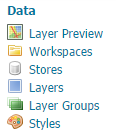
\includegraphics[width=0.25\textwidth]{Figures/Data.png}
	  \vspace{-10pt}
	\caption{\label{fig:data}Data section of navigator}
	  \vspace{-10pt}
\end{wrapfigure}
This section will give a step by step guide of how to create a visual geospacial representation using the pre-aggregated index of the example dataset. This will be done using GeoServer, specifically the GeoServer web administration interface. This section offers are concrete version of the deployment discussed in \Fref{sec:deployment}.

\Fref{fig:data} shows the \lstinline|Data| section of the navigator which can be found on the left hand side of the web administration interface. The links in this section will be used to navigate between different pages needed to configure the whole setup.

\subsubsection{Add Source}
A data source is added in the following manor:
\begin{enumerate}
	\item Click on the \lstinline|Stores| link in the \lstinline|Data| section shown in \Fref{fig:data}.
	\item The \lstinline|Stores| will open, the top of the page will look like \Fref{fig:newstore}, click on the \lstinline|Add new Store| link.
	\item A selection of different \lstinline|Vector Data Sources| is now available. Select \lstinline|NeoGeo Aggregate| as shown in \Fref{fig:storetype}. 
\end{enumerate}
\begin{figure}[h]
	\centering
	\subfigure[Add new store \label{fig:newstore}]{
		\raisebox{8mm}{
		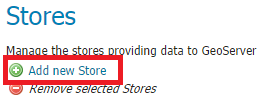
\includegraphics[scale=0.6]{Figures/AddNewStores.png} }}
	\subfigure[Select data source type \label{fig:storetype}]{
		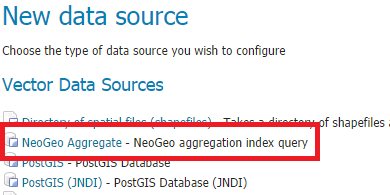
\includegraphics[scale=0.6]{Figures/StoreType.png} }
	\caption{Adding new \lstinline|Store| to GeoServer}
\end{figure}

\begin{enumerate}[resume]
	\item After selecting \lstinline|NeoGeo Aggregate| as \lstinline|Vector Data Source| a page like \Fref{fig:createstore} will open. Fill in all the fields as shown, some values may differ depending on how the database is setup. More exact information can be found in \Fref{sec:addingsource}.
	\item Once everything is filled out click the \lstinline|Save| button. This leads to page where \lstinline|Layers| can be published. However before that is done first the \lstinline|Style| should be imported.
\end{enumerate}

\begin{figure}[h!tb]
	\centering
		\begin{minipage}{0.5\textwidth}
			\centering 	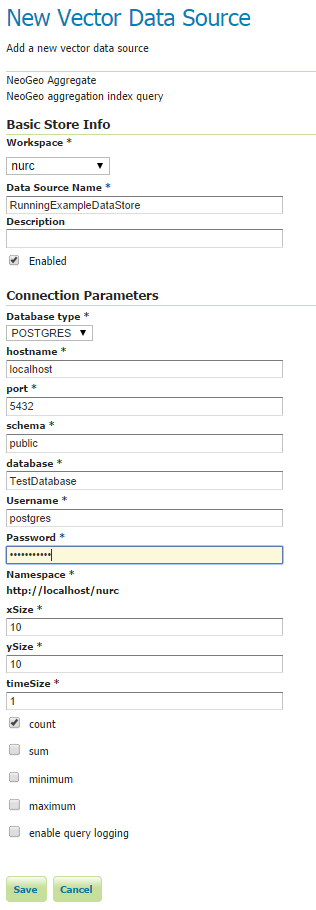
\includegraphics[width=.94\textwidth]{Figures/CreateStore.png}
			\caption{\label{fig:createstore}\lstinline|New Vector Data Source|}
		\end{minipage}\hfill
		\begin{minipage}{0.5\textwidth}
			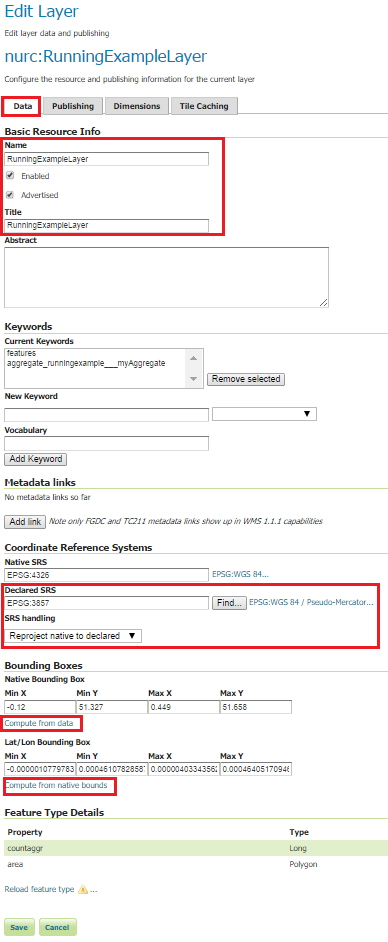
\includegraphics[width=1.11\textwidth]{Figures/EditLayer_Data.png}
			\caption{\label{fig:editlayerdata}\lstinline|Edit Layer| page}
		\end{minipage}
\end{figure}

\clearpage
\subsubsection{Import Style}
Importing a style is done as follows:
\begin{enumerate}[resume]
	\item Click on the \lstinline|Styles| link in the \lstinline|Data| section shown in \Fref{fig:data}.
	\item Click on the \lstinline|Add a new style| button which will go a page similar to \Fref{fig:styleimport} although empty.
	\item Import the \lstinline|RunningExampleSLD.xml| file by using the \lstinline|Choose File| button then the \lstinline|Upload...| link highlighted in red in \Fref{fig:styleimport}.
	\item Once the style has been upload the \lstinline|New style| page should look like \Fref{fig:styleimport}.
	\item Press the \lstinline|Save| button.
\end{enumerate}
The style used in this example has been imported in GeoServer and now the layer is ready to published.
\begin{figure}[h!]
	\centering
	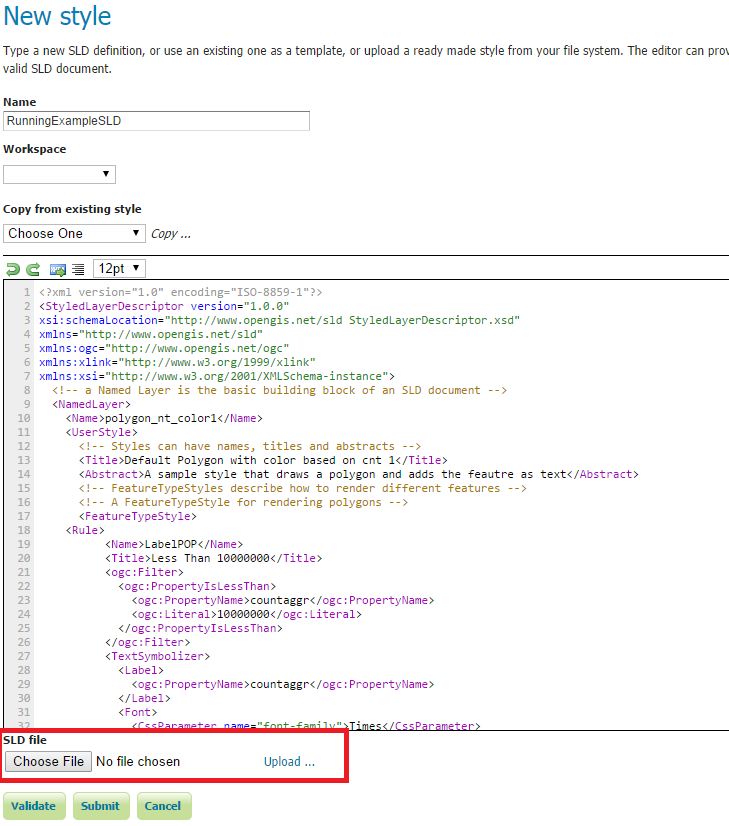
\includegraphics[scale=0.5]{Figures/NewStyleImport.png}
	\caption{\label{fig:styleimport}Importing SLD style from file}
\end{figure}

\pagebreak
\subsubsection{Create Layer}
\begin{figure}[h!]
	\centering
	\vspace{-15pt}
	\includegraphics[width=\textwidth]{Figures/Publishlayer.png}
	\vspace{-5pt}
	\caption{Publishing a \lstinline|Layer|\label{fig:publishlayer}}
\end{figure}
\noindent Creating a new layer is done as follows:
\vspace{10pt}

\begin{minipage}{.45\textwidth}
	\begin{enumerate}[resume]
		\item Click on the \lstinline|Layers| link in the \lstinline|Data| section shown in \Fref{fig:data}.
		\item This opens the \lstinline|Layers| page, here click on the \lstinline|Add a new resource| button. This open a page similar to \Fref{fig:publishlayer}.
		\item Select the \lstinline|Publish| action for the example layer.
		\item A page like \Fref{fig:editlayerdata} will open. Set highlighted fields to match \Fref{fig:editlayerdata}. More exact information about these fields can be found in \Fref{sec:addinglayers}.
		\item After the fields in the \lstinline|Data| are filled in, go to the \lstinline|Publishing| tab, see \Fref{fig:layerpublish}.
		\item Set the  default style to \lstinline|RunningExampleSLD| like in \Fref{fig:layerpublish}.
		\item Press the \lstinline|Save| button.
	\end{enumerate}
\end{minipage}\hfill
\begin{minipage}{.45\textwidth}
	\begin{figure}[H]
		\centering
		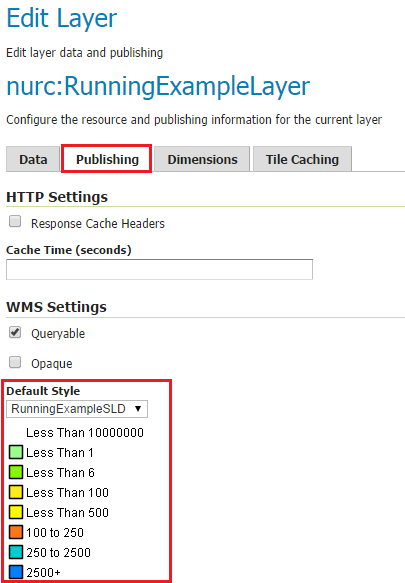
\includegraphics[width=\textwidth]{Figures/EditLayer_Publishing.png}
		\vspace{-5pt}
		\caption{Adding a \lstinline|Style| to the \lstinline|Layer| \label{fig:layerpublish}}
	\end{figure}
\end{minipage}

\vspace{10pt}
\noindent A layer for the example dataset has now been created and is ready to be viewed.


\pagebreak
\subsubsection{View Layer}
\begin{figure}[h!]
	\centering
	\vspace{-15pt}
	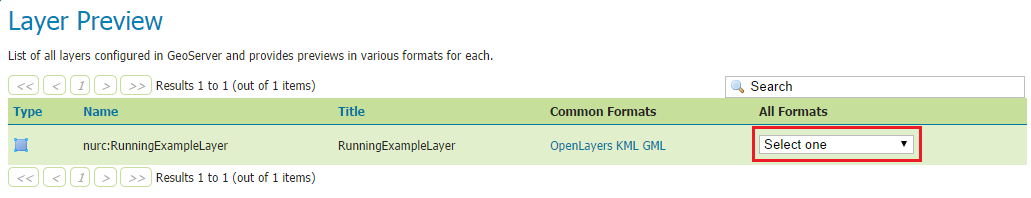
\includegraphics[width=\textwidth]{Figures/LayerPreview.png}
	\vspace{-25pt}
	\caption{Previewing a \lstinline|Layer|\label{fig:preview}}
\end{figure}
\noindent The final GeoServer step is to preview the layer. The preview only shows the highest granularity of the aggregation index. Getting a preview of a layer is done as follows:
\begin{enumerate}[resume]
	\item Click on the \lstinline|Layer Preview| link in the \lstinline|Data| section shown in \Fref{fig:data}.
	\item The \lstinline|Layer Preview| page opens which displays all viewable layers like in \Fref{fig:preview}.
	\item A preview format need to be selected from the drop-down menu highlighted in \Fref{fig:preview}.
	\item Select a \lstinline|WMS| preview format such as \lstinline|PNG|.
	\item A new web page will load (this might a few seconds depending on if the server side extension is enabled).
	\item The final result will look like \Fref{fig:result}.
\end{enumerate}
The layer which shows the example dataset is now complete. The values of each square in the layer is calculated using the pre-aggregate index of the dataset. See \ref{sec:clientsidedev} to learn how the layer can be used in combination with other tools such as OpenLayers\footnote{\url{http://openlayers.org/}} to create a dynamic map which updates data on the fly.
\begin{figure}[h!]
	\centering
	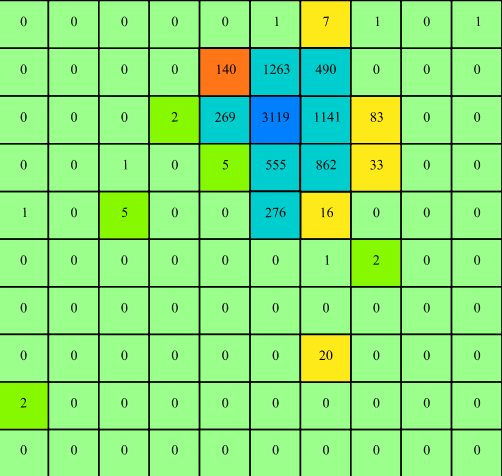
\includegraphics[width=0.45\textwidth]{Figures/FinalResult.png}
	\vspace{-5pt}
	\caption{Preview of whole dataset \label{fig:result}}
\end{figure}
\end{document}
